\documentclass[slidestop,compress,mathserif]{beamer}
%\documentclass[slidestop,compress,mathserif,handout]{beamer}

%\documentclass[xcolor=dvipsnames,handout]{beamer}
%\documentclass[xcolor=dvipsnames]{beamer}

%\documentclass[handout]{beamer}

%%% To get rid of solutions on handouts:
\newcommand{\soln}[1]{\textit{\textcolor{darkGray}{#1}}}				% For slides
%\newcommand{\soln}[1]{ }	% For handouts

% to get pausing to work properly on slides
\newcommand{\hide}[1]{#1}	% For slides
%\newcommand{\hide}[1]{ }	% For handouts


%\usepackage{multicol}
\usepackage{amsfonts}
%\usepackage[pdftex,dvipsnames]{color}
\usepackage{graphicx}
\usepackage{subfigure}
%\usepackage{picinpar}
\usepackage{pifont}
\usepackage{pgf,pgfarrows,pgfnodes}
%\usepackage{wasysym,manfnt,phaistos,empheq}
\usepackage[english]{babel}
\usepackage{pgfpages}
\usepackage{natbib}
\usepackage{hyperref}
\usepackage{multimedia}
%\usepackage{amsfonts,amstext,amssymb,amsbsy,amsopn,amsthm,eucal,latexsym,mathrsfs}
\usepackage{amsmath,amsfonts,amstext,amssymb,amsbsy,amsopn,amsthm,eucal,latexsym,mathrsfs}
\usepackage{ulem}
\usepackage{setspace}
\usepackage{array}
%\usepackage{rotating}
\usepackage{multirow}
\usepackage{verbatim}
\usepackage{multicol}

\setbeamertemplate{navigation symbols}{}

%\usepackage{tikz}
%\usetikzlibrary{arrows,shapes,trees,backgrounds}


%\setbeameroption{show notes on second screen}
%\setbeameroption{show notes}
%\setbeameroption{show only notes}

\definecolor{links}{HTML}{2A1B81}
\hypersetup{colorlinks,linkcolor=,urlcolor=links}

\newtheorem*{principle}{Inscrutibility Principle}
\newtheorem*{punchline}{Punch Line}
\newtheorem{defn}{Definition}

\definecolor{Scarlet}{RGB}{140,17,17}
\definecolor{VassarRed}{RGB}{128,0,0}

% "dinglist" environment
  \renewenvironment{dinglist}[2][blue]
  {\begin{list}{\textcolor{blue}{\ding{#2}}}{}}{\end{list}}
  % Symbol definitions for these lists
  \newcommand{\DingListSymbolA}{43}
  \newcommand{\DingListSymbolB}{243}
  \newcommand{\DingListSymbolC}{224}
  \newcommand{\DingListSymbolD}{219}
  \newcommand{\DingListSymbolCheck}{52}
  \newcommand{\DingListSymbolCross}{56}


  \newenvironment{ballotenv}
{\only{%
\setbeamertemplate{itemize item}{\ding{45}}%
\setbeamertemplate{itemize subitem}{\ding{46}}%
\setbeamertemplate{itemize subsubitem}{\ding{46}}}} {}
\setbeamertemplate{itemize item}{\ding{49}}
\setbeamertemplate{itemize subitem}{\ding{47}}
\setbeamertemplate{itemize subsubitem}{\ding{47}}


%User defined colors: See colors section
\xdefinecolor{oiBlue}{rgb}{0.15, 0.35, 0.55}
\xdefinecolor{gray}{rgb}{0.5, 0.5, 0.5}
\xdefinecolor{darkGray}{rgb}{0.3, 0.3, 0.3}
\xdefinecolor{darkerGray}{rgb}{0.2, 0.2, 0.2}
\xdefinecolor{rubineRed}{rgb}{0.89,0,0.30}
\xdefinecolor{linkCol}{rgb}{0.11,0.49,0.95}	
\xdefinecolor{irishGreen}{rgb}{0,0.60,0}	
\xdefinecolor{darkturquoise}{rgb}{0.44, 0.58, 0.86}
\definecolor{lightGreen}{rgb}{0.533,0.765,0.42}
\xdefinecolor{Regalia}{HTML}{522D80}
\xdefinecolor{ClemsonOrange}{HTML}{EA6A20}

\definecolor{duke@LightGrey}{RGB}{200,200,200}\definecolor{DarkGreen}{RGB}{0,100,0}
\definecolor{Oranges}{RGB}{255,127,0}
\definecolor{LightGray}{RGB}{211,211,211}

%\setbeamertemplate{footline}{%
%  \raisebox{5pt}{\makebox[\paperwidth]{\hfill\makebox[10pt]{\scriptsize\insertframenumber}}}}

\setbeamercolor{equation background}{fg=black,bg=duke@LightGrey}
  % Boxed equation
  \newcommand{\eqbox}[2][0.6]{%
  \centerline{
  \begin{beamerboxesrounded}[lower=equation background,width=#1\hsize,shadow=true]{}
\parbox{#1\hsize}{%
      \[
        \textcolor{black} {#2}
      \]}
  \end{beamerboxesrounded}
}}

\AtBeginSection[] {
  \begin{frame}<beamer>\frametitle{Outline}
    \tableofcontents[currentsection,hideothersubsections]
  \end{frame}
}
%
%
%\AtBeginSubsection[] {
%  \begin{frame}<beamer>\frametitle{Outline}
%    \tableofcontents%[currentsection,currentsubsection]
%  \end{frame}
%}

%\usecolortheme[RGB={82,45,128}]{structure}
%\usecolortheme[RGB={162,80,22}]{structure}
\usecolortheme[RGB={128,0,0}]{structure}
\usetheme[secheader]{Boadilla}
%\usetheme[height=7mm]{Rochester}
%\usetheme{Copenhagen}
%\usetheme{Antibes}
%\usecolortheme{seahorse}
%\usecolortheme{crane}
%\usecolortheme{rose}
%\usefonttheme[onlylarge]{structurebold}
%\usefonttheme[onlymath]{serif}



\def\diag{{\rm diag}}


\def\E{\mathbb{E}}
\def\Prob{\mathbb{P}}
\def\argmin{{\rm argmin}}
\def\argmax{{\rm argmax}}
\def\Def{\stackrel{def}{=}}


\newtheorem{assumption}{Assumptions}
\newtheorem*{proposition}{Proposition}
\newtheorem*{remark}{Remark}



%\setbeamercolor{disc title}{bg=oiBlue!40!white!60,fg=blue}
\setbeamercolor{disc body}{bg= Regalia!20!white!80,fg= Regalia!80!black!90}

\setbeamercolor{clicker ungraded title}{bg=irishGreen!80!white!50,fg=irishGreen!30!black!90}
\setbeamercolor{clicker ungraded body}{bg=irishGreen!20!white!80,fg=irishGreen!30!black!90}

\setbeamercolor{clicker review title}{bg=gray!80!white!80,fg=oiBlue!80!black!90}
\setbeamercolor{clicker review body}{bg=gray!30!white!90,fg=oiBlue!80!black!90}

\setbeamercolor{code body}{bg=gray!20!white!80,fg=black}


% Custom commands
\newcommand{\degree}{\ensuremath{^\circ}}
\newcommand{\Note}[1]{
\rule{2.5cm}{0.25pt} \\ \textit{\scriptsize {\textcolor{rubineRed}{Note:} \textcolor{gray}{#1}}}}
\newcommand{\ct}[1]{
\vfill
{\tiny #1}}
\newcommand{\Remember}[1]{\textit{\scriptsize{\textcolor{orange}{Remember:} \textcolor{gray}{#1}}}}
\newcommand{\red}[1]{\textit{\textcolor{rubineRed}{#1}}}
\newcommand{\pink}[1]{\textit{\textcolor{rubineRed!90!white!50}{#1}}}
\newcommand{\green}[1]{\textit{\textcolor{irishGreen}{#1}}}
\newcommand{\webURL}[1]{\urlstyle{same}\textit{\textcolor{linkCol}{\url{#1}}} }
\newcommand{\webLink}[2]{\href{#1}{\textcolor{linkCol}{{#2}}}}
\newcommand{\mail}[1]{\href{mailto:#1}{\textit{\textcolor{linkCol}{#1}}}}
\newcommand{\hl}[1]{\textit{\textcolor{oiBlue}{#1}}}
\newcommand{\hlGr}[1]{\textit{\textcolor{lightGreen}{#1}}}
\newcommand{\mathhl}[1]{\textcolor{oiBlue}{\ensuremath{#1}}}
\newcommand{\ex}[1]{\textcolor{blue}{{{\small (#1)}}}}
\newcommand{\disc}[1]{
\begin{beamerboxesrounded}[shadow = true, lower = disc body, upper = disc title]{}
#1
\end{beamerboxesrounded}
}

\newcommand{\cl}[1]{
\begin{beamerboxesrounded}[shadow = true, lower = clicker ungraded body, upper = clicker ungraded title]{Question}
$\:$ \\
#1
\end{beamerboxesrounded}
}

\newcommand{\clR}[1]{
\begin{beamerboxesrounded}[shadow = true, lower = clicker review body, upper = clicker review title]{\red{Review question} }
$\:$ \\
#1
\end{beamerboxesrounded}
}

\newcommand{\formula}[2]{
\begin{beamerboxesrounded}[shadow = true, lower = white, upper = clicker review body]{#1}
#2
\end{beamerboxesrounded}
$\:$ \\
}

\newenvironment{twocol}[4]{
\begin{columns}[c]
\column{#1\textwidth}
#3
\column{#2\textwidth}
#4
\end{columns}
}


\newenvironment{slot}[2]{
\begin{array}{c}
\underline{#1} \\
#2
\end{array}
}

\newcommand{\pr}[1]{
\left( #1 \right)
}

\newcommand{\solnMult}[1]{
\item[] \vspace{-0.59cm}
\only<beamer| beamer:1>{\item #1}
\soln{\only<2->{\item \red{#1}}}
}

%\newcommand{\codechunk}[1]{
%\begin{beamerboxesrounded}[shadow = true, lower = code body]{}
%{\small #1}
%\end{beamerboxesrounded}
%}

% Change margin

\newenvironment{changemargin}[2]{%
\begin{list}{}{%
\setlength{\topsep}{0pt}%
\setlength{\leftmargin}{#1}%
\setlength{\rightmargin}{#2}%
\setlength{\listparindent}{\parindent}%
\setlength{\itemindent}{\parindent}%
\setlength{\parsep}{\parskip}%
}%
\item[]}{\end{list}}

% Footnote

\long\def\symbolfootnote[#1]#2{\begingroup%
\def\thefootnote{\fnsymbol{footnote}}\footnote[#1]{#2}\endgroup}

% Commands from the book
\newenvironment{data}[1]{\texttt{#1}}{}
\newenvironment{var}[1]{\texttt{#1}}{}
\newenvironment{resp}[1]{\texttt{#1}}{}






%%%%%%%%%%%%%%%%%%%%%%%%%%%%%%%%%%%%%%%%%%%%%%%%%%%%%%%%%%%%%%%%%%%%%%%%%%%%%%%%%%%%%%%%%%%%%%%

\title[Chapter 4 part 2]{Chapter 4 part 2}
\subtitle{Discrete Random Variables}

%%%%%%%%%%%%%%%%%%%%%%%%%%%%%%%%%%%%%%%%%%%%%%%%%%%%%%%%%%%%%%%%%%%%%%%%%%%%%%%%%%%%%%%%%%%%%%%


\author[Jingchen (Monika) Hu] % (optional, use only with lots of authors)
{Jingchen (Monika) Hu}
% - Give the names in the same order as the appear in the paper.
% - Use the \inst{?} command only if the authors have different
%   affiliation.

\institute[Vassar] % (optional, but mostly needed)
{Vassar College}
% - Use the \inst command only if there are several affiliations.
% - Keep it simple, no one is interested in your street address.

\date[MATH 241] % (optional, should be abbreviation of conference name)
{MATH 241}
% - Either use conference name or its abbreviation.
% - Not really informative to the audience, more for people (including
%   yourself) who are reading the slides online

\subject{MATH 241}
% This is only inserted into the PDF information catalog. Can be left
% out.



% If you wish to uncover everything in a step-wise fashion, uncomment
% the following command:

%\beamerdefaultoverlayspecification{<+->}


\begin{document}




%%%%%%%%%%%%%%%%%%%%%

% Title Page

\begin{frame}%[plain]
\titlepage
\end{frame}

%%%%%%%%%%%%%%%%%%%%%
%\addtocounter{framenumber}{-1}
%
%\begin{frame}\frametitle{Annoucement}
%
%\begin{itemize}
%\item HW3: \red{due now!}
%\item HW4: \red{due Tuesday, Sept 30th}
%\end{itemize}
%
%
%\end{frame}
%
%



%%%%%%%%%%%%%%%%%%%%%%%%%%%%%%%%%%%%%%%%%%
\section{Variance}
%%%%%%%%%%%%%%%%%%%%%%%%%%%%%%%%%%%%%%%%%%

\begin{frame}\frametitle{Variance}

\begin{itemize}
\item Expected value (or mean) $\mu = E[X]$ yields the weighted average of the possible values of X
\end{itemize}

\begin{defn}
\hl{Variance} measures the variation (or spread) of these values
\[\sigma^2 = Var(X) = E\left[ (X-E(X))^2\right] = E\left[(X-\mu)^2 \right] \]
This holds for all random variable $X$ (not necessary discrete random variable).
\end{defn}

\begin{itemize}
\item One common simplification:
\[
Var(X) 	  =  E(X^2)-\mu^2
\]
\end{itemize}


\end{frame}

%%%%%%%%%%%%%%%%%%%%%%%%%%%%%%%%%%%%%%%%%%
\begin{frame}\frametitle{Standard deviation}

\begin{defn}
\hl{Standard Deviation} is the square root of the variance
\[\sigma = SD(X) = \sqrt{Var(X)}\]
\end{defn}

\end{frame}


%%%%%%%%%%%%%%%%%%%%%%%%%%%%%%%%%%%%%%%%%%
\begin{frame}
\cl{Let the random variable $X$ denote the GP a certain student will earn in this class. Suppose its pmf is
\[ p(0) = 0.05, \quad p(1) = 0.05, \quad p(2) = 0.3, \quad p(3) = 0.4\]
Calculate their GP variance $Var[X]$.
}

\pause
\[
Var(X) 	  =  E(X^2)-(E[X])^2
\]
First compute $p(4) = 1 - p(0) - p(1) - p(2) - p(3) = 0.2$.\\
Then compute $E[X]$ and $E[X^2]$
\[ E[X] = 0 \times 0.05 + 1 \times 0.05 + 2 \times 0.3 + 3 \times 0.4 + 4 \times 0.2 = 2.65 \]
\[ E[X^2] = 0^2 \times 0.05 + 1^2 \times 0.05 + 2^2 \times 0.3 + 3^2 \times 0.4 + 4^2 \times 0.2 = 8.05\]
Finally we have 
\[Var[X] = E(X^2)-(E[X])^2 = 8.05 - 2.65^2 = 1.0275\]
\end{frame}


%%%%%%%%%%%%%%%%%%%%%%%%%%%%%%%%%%%%%%%%%%
\begin{frame}
\cl{Find $Var(X)$ if
\[
P(X = a) = p = 1 - P(X = b)
\]
}

\pause
\[
Var(X) 	  =  E(X^2)-(E[X])^2
\]
First compute $E[X]$ and $E[X^2]$
\[ E[X] = a \times p + b \times (1 - p) \]
\[ E[X^2] = a^2 \times p + b^2 \times (1 - p)\]
Then we have 
\[Var[X] = E(X^2)-(E[X])^2 = a^2 \times p + b^2 \times (1 - p) - \left(a \times p + b \times (1 - p)\right) ^ 2\]
\end{frame}




%%%%%%%%%%%%%%%%%%%%%%%%%%%%%%%%%%%%

%%%%%%%%%%%%%%%%%%%%%%%%%%%%%%%%%%%%

\begin{frame}
\frametitle{Properties of variance}

$Var(X) \geq 0$
\begin{itemize}
\item $Var(X) = 0$ if and only if $X$ is a constant.
\end{itemize}


\vspace{0.2cm}
If $a$ and $b$ are constants, then
\[ Var(aX+b) = a^2 Var(X) \]


\begin{itemize}
\item \[ Var(aX) = a^2 Var(X) \]
\item \[ Var(X + b) =  Var(X) \]
\item \[ Var(b) = 0 \]
\end{itemize}

\end{frame}


%%%%%%%%%%%%%%%%%%%%%%%%%%%%%%%%%%%%%%%%%%
\begin{frame}
\cl{If $E[X] = 1$ and $Var(X) = 5$, find (a) $E[(2 + X)^2]$, (b) $Var(4 + 3X)$.
}

\pause
\[
Var(X) 	  =  E(X^2)-(E[X])^2
\]
\[
E[aX + b] = aE[X] + b; Var(aX+b) = a^2 Var(X)
\]

Part (a):
\begin{eqnarray*}
E[(2 + X)^2] &=& Var(2 + X) + (E[2 + X]^2) \\
&=& Var(X) + (2 + E[X])^2 = 5 + 9 = 14
\end{eqnarray*}

Part (b)
\begin{eqnarray*}
Var(4 + 3X) = 3^2 \times Var(X) = 9 \times 5 = 45
\end{eqnarray*}

\end{frame}

%%%%%%%%%%%%%%%%%%%%%%%%%%%%%%%%%%%%
\section{Bernoulli distribution and Binomial distribution}
%%%%%%%%%%%%%%%%%%%%%%%%%%%%%%%%%%%%
\begin{frame}\frametitle{Bernoulli distribution}

A trial has two outcomes: success (1) or failure (0). \\
Let random variable $X$ be the number of success in a single trial.

\begin{defn}
Random variable $X$
has a \hl{Bernoulli distribution}, if
\[
P(X = 1) = p, \quad P(X = 0) = 1-p
\]
where $0 \leq p \leq 1$ is the probability of a success.
\end{defn}

\twocol{0.78}{0.22}{
\begin{itemize}
\item The pmf of Bernoulli distribution
\[ X \sim \text{Ber}(p) \Longleftrightarrow\ p(1) = p, \ p(0) = 1-p \]


\item Found by Swiss mathematician Jacob Bernoulli.
\end{itemize}
}
{
\begin{center}
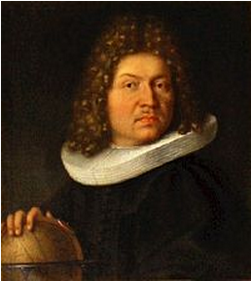
\includegraphics[width = \textwidth]{figures/Jacob_Bernoulli}
\end{center}
}

\end{frame}

%%%%%%%%%%%%%%%%%%%%%%%%%%%%%%%%%%%%%%%%%%
\begin{frame}\frametitle{Recap}

Variance $\sigma^2$
\begin{itemize}
\item \textbf{For all random variable}
\[
Var(X) = E[(X - \mu)^2] = E[X^2] - \mu^2
\]
\vspace{2mm}
\item \textbf{Linear function}
\[Var(aX+b) = a^2 Var(X)\]
\item \textbf{Constants}
\[Var(c) = 0\]
\end{itemize}

Standard deviation
\[SD(X) = \sqrt{Var(X)}\]

Bernoulli distribution
\[p(1) = p, \quad p(0) = 1-p\]
\[\mu  = p, \quad \sigma^2 = p(1-p)\]

\end{frame}

%%%%%%%%%%%%%%%%%%%%%%%%%%%%%%%%%%%%

%%%%%%%%%%%%%%%%%%%%%%
%\begin{frame}{Outline}
%%\tableofcontents[hideallsubsections,pausections]
%\tableofcontents[hideallsubsections]
%\end{frame}


%%%%%%%%%%%%%%%%%%%%%%%%%%%%%%%%%%%%%%%%%%
\begin{frame}\frametitle{Binomial distribution}
\begin{defn}
Define $X$ to be the \emph{number of successes} in a \emph{fixed number} $n$
of \emph{independent trials} with the \emph{same probability of success} $p$ as having a \hl{Binomial distribution}.


Then the pmf of $X$ is $P(X = k) = P(\text{getting } k \text{ successes in } n \text{ trials})$
 \vspace{-0.3cm}
\[ X \sim \text{Bin}(n,p) \Longleftrightarrow \ p(k) = {n \choose k} p^k(1-p)^{n-k}, \quad k = 0, 1, \ldots, n\]

\end{defn}




\end{frame}


%%%%%%%%%%%%%%%%%%%%%%%%%%%%%%%%%%%%%%%%%%
\begin{frame}%\frametitle{Pmf of Binomial distribution: uni-modeal}
\cl{Let $X$ be the number of 6 obtained when roll four fair 6-sided dice simultaneously.
Its pmf is.
\begin{center}
\begin{tabular}{c | c | c | c | c | c }
$x$				& $0$			& $1$			& $2$			& $3$			& $4$			\\
\hline
$p(x)$			&$0.4823$		&$0.3858$ 		&$0.1157$ 		&$0.0154$ 		&$0.0008$ 	\\
\end{tabular}
\end{center}
Find its cdf $F(x)$.
}
%\vspace{0.5cm}
\pause
%\invisible{
\[
F(x) = 	\begin{cases}
		0 	& \text{ if } x < 0\\
		0.4823 	& \text{ if } 0 \leq x < 1\\
		0.8681 	& \text{ if } 1 \leq x < 2\\
		0.9838 	& \text{ if } 2 \leq x < 3\\
		0.9992 	& \text{ if } 3 \leq x < 4\\
		1 		& \text{ if } x \geq 4\\
		\end{cases}
\]

%}


\end{frame}


%%%%%%%%%%%%%%%%%%%%%%%%%%%%%%%%%%%%


\begin{frame}
\frametitle{}

\cl{I drink a cup of coffee everyday. About $80\%$ of the time I buy coffee from CraftedKup,
about $20\%$ of the time from the Starbucks. Compute the probability I drink 4 cups of Starbucks coffee in 10 days. }

\pause
\[
{10 \choose 4} \times 0.2^4 \times 0.8^6 = 210 \times  0.2^4 \times 0.8^6 = 0.088
\]

\end{frame}

%%%%%%%%%%%%%%%%%%%%%%%%%%%%%%%%%%%%%%%%%
\begin{frame}\frametitle{Pmf of Binomial distribution: uni-modal}

\vspace{-0.5cm}
\begin{center}
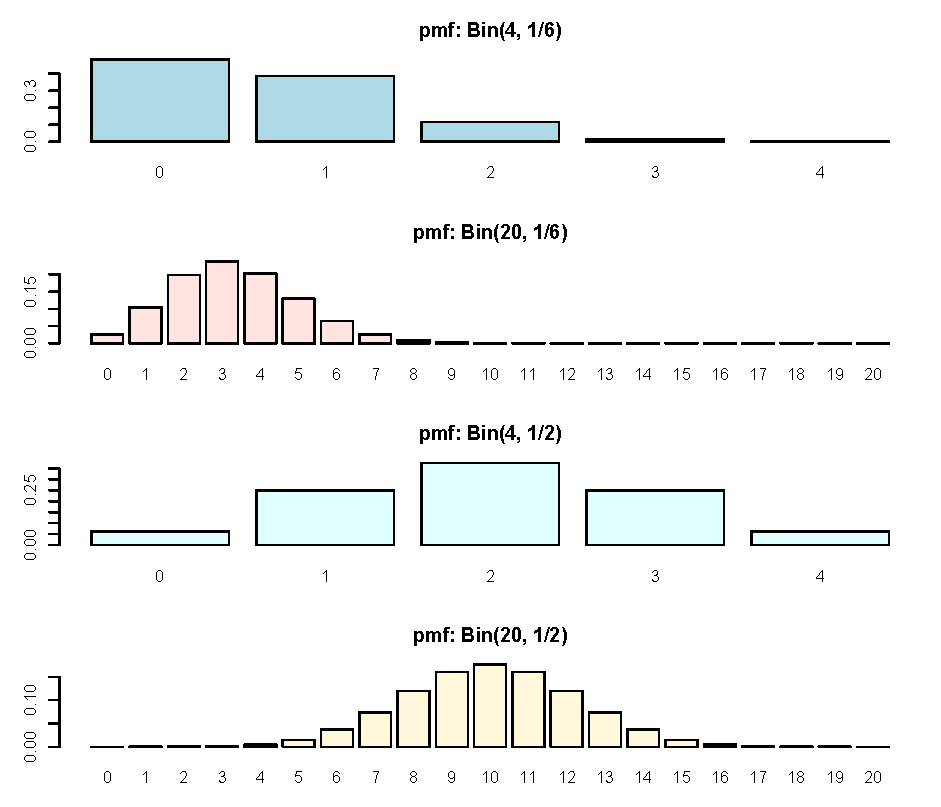
\includegraphics[scale = 0.6]{figures/pmf2}
\end{center}

\end{frame}


%%%%%%%%%%%%%%%%%%%%%%%%%%%%%%%%%%%%%
%
%\begin{frame}\frametitle{Mode of Binomial distribution}
%
%\begin{itemize}
%\item $X \sim \text{Bin}(n, p)$ and $p \in (0, 1)$. Then as $k$ goes from $0$ to $n$,
%\begin{align*}
%& p(k) \text{ increases  for } 0 \leq k \leq (n+1)p\\
%& p(k) \text{ decreases   for } (n+1)p < k \leq n
%\end{align*}
%\end{itemize}
%\pause
%\red{Recall the Binomial Theorem $(a + b)^n = \sum_{k=0}^n {n \choose k} a^k b^{n-k}$}
%
%
%\end{frame}

%%%%%%%%%%%%%%%%%%%%%%%%%%%%%%%%%%%%%%%%%%
\begin{frame}\frametitle{Binomial pmf is valid (or well-defined)} %$p(k) = {n \choose k} p^k (1-p)^{n-k}$}

\begin{itemize}
\item Positive: for any $x \in \mathbb{R}$
\[p(x) \geq 0\]
\item Total one ({\color{red}required}):
 \[\sum_{k = 0}^n p(k) = 1\]
\red{Recall the Binomial Theorem $(a + b)^n = \sum_{k=0}^n {n \choose k} a^k b^{n-k}$}
$$\sum_{k = 0}^n p(k) = \sum_{k = 0}^n {n \choose k} p^k(1-p)^{n-k} = [p+(1-p)]^n = 1^n = 1$$

\end{itemize}

\end{frame}
%%%%%%%%%%%%%%%%%%%%%%%%%%%%%%%%%%%%%%%%%%
\begin{frame}\frametitle{Mean of Binomial random variable}

Toss a coin $n$ times, each toss has prob $p$ being a head. On average,
total number of heads equals $np$.\\

\[E[X] = np \]

Check textbook page 131 for the derivation ({\color{red}not required}).

\end{frame}

%%%%%%%%%%%%%%%%%%%%%%%%%%%%%%%%%%%%%%%%%%
\begin{frame}\frametitle{Properties of Binomial distribution}

\begin{itemize}
\item Variance
\[Var[X] = np(1-p) \]
Check textbook page 132 for the derivation ({\color{red}not required}).


\vfill
\item If we have independent Bernoulli random variable's $X_1, X_2, \ldots, X_n$ with the same probability of success $p$, then
their sum has a Binomial distribution
\[
X = X_1 + X_2 + \cdots + X_n \sim \text{Bin}(n, p)
\]


\end{itemize}

\end{frame}

%%%%%%%%%%%%%%%%%%%%%%%%%%%%%%%%%%%%%
%%%%%%%%%%%%%%%%%%%%%%%%%%%%%%%%%%%%%%%%%%
\begin{frame}\frametitle{Recap}

Binomial distribution $X \sim \text{Bin}(n,p) $
\[ p(k) = {n \choose k} p^k(1-p)^{n-k}\]
\begin{itemize}
\item mean $\mu = np$
\item variance $\sigma^2 = np(1-p)$
%\item Bernoulli distribution: $n=1$
\end{itemize}


\end{frame}

%%%%%%%%%%%%%%%%%%%%%%%%%%%%%%%%%%%%

\begin{frame}\frametitle{}

\cl{Random variable $X \sim \text{Binom}(n,p)$, and the value of $n$ is fixed.
For any fixed $n$, find $p$ such that the distribution of $X$ has the largest spread.}

%\invisible{
\pause\vspace{0.5cm}
Variance (or standard deviation) is a measurement of spread.
\[ \sigma^2 = np(1-p) \]
\pause
To find the $\hat{p}$ that maximize the spread, i.e., find the root of the derivative
\begin{align*}
\frac{d \sigma^2}{d p} & = n (1-p + (-p)) = 0\\
& \Longrightarrow \hat{p} = 1/2
\end{align*}


%}

\end{frame}


%%%%%%%%%%%%%%%%%%%%%%
%\begin{frame}{Outline}
%%\tableofcontents[hideallsubsections,pausections]
%\tableofcontents[hideallsubsections]
%\end{frame}
%
%%%%%%%%%%%%%%%%%%%%%%%%%%%%%%%%%%%%%%%%%%


\end{document} 